Come si trasmettono le informazioni da un router all'altro fino agli endpoint è opera del livello \textit{datalink}. \\
Questo livello si appoggia sul concetto di \textit{trama} (o \textit{frame}), un percorso seguito dal flusso, che inizia e finisce su due estremi. Dunque i protocolli a livello di collegamento si occupano del trasporto di datagrammi lungo un singolo canale di comunicazione. Offre diversi servizi:
\begin{itemize}
	\item rilevamento e correzioni di errori;
	\item condivisione di canali broadcast, offrendo accessi multipli;
	\item servizio di gestione degli indirizzi di livello link;
	\item trasferimento dati affidabili, con controllo del flusso.
\end{itemize}
Il livello di rete è implementato sugli \textit{adaptor} (adattatore di rete, o scheda di rete, \textit{NIC} - \textit{network interface card}), che comunicano l'uno con l'altro - stabilendo una trama per raggiungersi - e che devono rispettare gli standard appena esposti. \\
Si tratta di una combinazione di hardware, software e firmware. \\
Accetta soltanto degli stream di raw bit (flussi di sequenze di bit) e cerca di consegnarlo a destinazione: ciononostante la comunicazione non è necessariamente priva di errori. Per gestire un numero multiplo di flussi di informazioni, divide lo stream in un numero variabile di trama (\textit{framing}) e elabora il checksum per ogni trama (per ovviare a problemi di generazione e correzione errori). \\
Lo split viene applicato ogni \textit{n} caratteri, e ciascun flusso è delimitato da dei caratteri speciali: \textit{DLE STX} (\textit{Data Link Escape Start of TeXt}) e DLE ETX (\textit{Data Link Escape End of TeXt}). Qualora dovesse essere inviata esattamente la stringa utilizzata come escape, viene aggiunto un \textit{DLE} per eliminare ambiguità. \\
Possono essere poi utilizzati degli approcci meno generici, come il sistema \textit{Manchester}.

\section{Rilevamento e correzione di errori, controllo del flusso}
\paragraph{Consegna affidabile}
La consegna affidabile è garantita attraverso lo stesso sistema già utilizzato sul livello di trasporto, gli \textit{ack}; ciononostante, è risulta necessaria soltanto nei collegamenti soggetti ad elevati tassi di errori (e.g., collegamenti wireless, e così via \ldots), ma non su quelli che presentano un basso numero di errori sui bit (e.g., fibra ottica, e così via \ldots).
\paragraph{Rilevamento degli errori}
Tra i dati trasmessi, vi sono due blocchi fondamentali:
\begin{enumerate}
	\item \textit{EDC}: bit - ridondanti - di \textit{error detection and correction};
	\item \textit{D}: dati protetti dal controllo di errori - eventualmente accompagnati da campi header.
\end{enumerate}
Ovviamente la rilevamento di errori non è affidabile al 100\%: si potrebbero raramente non rilevare alcuni errori, in maniera inversamente proporzionale alla dimensione alla dimensione dell'\textit{EDC} utilizzata. \\
Nel rilevamento di errori, si utilizza il calcolo della distanza di \textit{Hamming}, attraverso cui è possibile determinare in quanti bit differiscano due parole di codice. Sostanzialmente, si esegue lo \textit{XOR} tra le parole e poi si conta il numero di 1 nel risultato: il numero di posizioni nelle quali le due parole di codice differiscono determina la loro distanza di \textit{Hamming}. Se due parole hanno distanza di \textit{Hamming} \textit{d}, ci vorranno \textit{d} operazioni sui singoli bit per tramutare una parola di codice nell'altra: per come sono utilizzati i bit di ridonanza, se la lunghezza delle parole di codice è $n=m+4$, sono possibili $2^m$ messaggi dati validi, ma non tutte le $2^n$ parole di codice. Dunque la distanza di \textit{Hamming} di un codice è la minima distanza di \textit{Hamming} tra le due parole di codice. Ancora, per rilevare \textit{d} errori occorre un codice con distanza di \textit{Hamming} $d+1$, mentre per correggerli serve un codice con distanza di \textit{Hamming} $2d+1$. \\
Alternativa al sistema di riconoscimento di errori tramite \textit{bit di parità} è il \textit{checksum}: il dato da trasmettere viene trattato come una sequenza di numeri interi da $k$ bit. Il \textit{checksum} è il risultato della somma di questi numeri da $k$ bit, per poi utilizzare i bit del risultato come bit per la rilevazione di errori.

\subsection{CRC (Cyclic Redundancy Check)}
Vengono visti i bit, \textit{D}, come un numero binario. Viene scelto un polinomio generatore di grado $r+1$ (una sequenza binaria in cui il primo elemento è sempre 1), del quale sono a conoscenza sia la sorgente che la destinazione. L'obiettivo è trovare un numero \textit{r} di bits \textit{CRC} di ridondanza \textit{R}: viene calcolato così che $<D,R>$ (concatenazione) sia esattamente divisibile per \textit{G} (in modulo 2). Il ricevente conosce \textit{G}, e divide $<D^1,R^1>$ per \textit{G} e controlla che il resto di questa operazione sia proprio 0, il che gli garantisce che l'informazione non contenga errori. \\
Questo approccio è molto utilizzato in internet.

\section{Protocolli di accesso multiplo}
Due tipologie di link:
\begin{itemize}
	\item \textit{punto-punto} (sorgente-destinazione): due nodi collegati da un link (come nel caso dei \textit{dialup PPP} e \textit{link ethernet}). Nessun rischio di collisione e viene sfruttata l'intera capacità del mezzo trasmissivo, dedicata a due soli dispositivi;
	\item \textit{broadcast}: il mezzo trasmissivo viene condiviso tra più nodi (come nel vecchio ethernet con topologia a \textit{bus}, nell'\textit{HFC}, nelle reti satellitari e nell \textit{802.11 wirelless} - wifi). Aperto a rischio di collissioni e il collegamento è condiviso tra varie coppie di dispositivi.
\end{itemize}
Se tutti i nodi sono liberi di contattare un mezzo trasmittivo, ci si apre al rischio di eventuali collisioni, motivo per cui è necessario introdurre delle regole. Occorre inoltre gestire il problema delle diverse potenze di trasmissione, noto come \textit{capture effect}: se c'è una grossa differenza di potenza tra due trasmissioni distinte, quello che trasmette con minore potenza non compromette completamente il primo; infatti, la sua trasmissione diventa sostanzialmente un \textit{rumore di fondo}, nonostante potrebbe rappresentare un caso di collisione.

\subsection{Mezzo condiviso}
Un protocollo di accesso multpilo è un protocollo che regolamenta l'utilizzo del mezzo trasmissivo per evitare fenomeni di collisione. \\
Le caratteristiche desiderabili sarebbero:
\begin{itemize}
	\item Data un'unica stazione di trasmissione, questa possa avere il massimo della capacità trasmissiva;
	\item Dato un numero variabile di nodi, questi possano avere una distribuzione equa della potenza di trasmissione dedicata a ciascuno;
	\item Un approccio decentralizzato: non voglio ci sia un elemento a coordinare la trasmissione e che non ci sia la necessità di sincronizzazione di orologi (perché ha un costo);
	\item Sia il più semplice possibile.
\end{itemize}
Protocolli MAC effettivamente proposti:
\begin{itemize}
	\item \textit{Channel Partitioning}: si divide il canale in sezioni, ognuna dedicata a ciascun nodo
	\begin{itemize}
		\item \textit{TDMA} (\textit{Time Division Multiple Access}): dispositivi hanno una visione comune del tempo, diviso in \textit{trame} (divise in tanti slot quanti sono i nodi che possono utilizzare la stessa stazione di trasmissione). All'interno del tempo di trama viene data la possibilità a un nodo di trasmettere con uno slot di una trama. Richiede sincronizzazione e occorre una porzione di banda detta \textit{banda di guardia}, utilizzata per separare le date sezioni;
		\item \textit{FDMA} (\textit{Frequency Division Multiple Access}): la banda viene divisa in tante sezioni di frequenza quanti sono gli utenti, in modo tale che ciascuno abbia le sue risorse, ma equa capacità di banda;
		\item \textit{CDMA}.
	\end{itemize}
	Sicuramente si tratta in entrambi i casi di una divisione equa, una soluzione - non ideale - di struttura decentralizzata e i protocolli sono semplici, ma non è possibile trasmettere a potenza massima 
	\item \textit{Random Access}: non diviso, permette collisioni:
	\begin{itemize}
		\item \textit{Slotted ALOHA}: la trasmissione viene divisa in frame di tempo uguali, gli slot; se due o più nodi trasmettono in uno stesso slot, si verifica una collisione, per la quale si reagirà trasmettendo nel prossimo slot. Mentre quando si trasmette lo si fa a potenza massima e per quanto si tratti di un algoritmo semplice, è soltanto parzialmente efficace, perché si verificano troppo spesso collisioni e troppo tempo viene speso senza effettiva trasmissione. Altro problema è il fatto che tutti i nodi devono essere esattamente sincronizzati sulla cadenza di ciascuno slot. Secondo un'analisi sull'efficienza, nel caso migliore, trasmette nel 37\% del tempo.
		\item \textit{Pure (unslotted) ALOHA}: se c'è qualcosa da trasmettere, viene fatto senza precauzioni, per un arco di tempo fisso. Se si presenta una collisione aspetto un arco di tempo fisso e poi avviene un nuovo tentativo. Il problema è che, mentre non c'è più sincronizzazione sulla cadenza tra uno slot e l'altro, si presenta perciò una sovrapposizione tra trasmissioni di diversi nodi. In questo caso, secondo un'analisi sull'efficienza, risulta trasmettere - nel caso migliore - nel 18\% del tempo.
		\item \textit{CSMA} (\textit{Carrier Sense Multiple Access}): una nuova estensione dell'\textit{ALOHA}. In questo caso, prima di trasmettere si verifica che non ci sia nessun altro nodo in trasmissione. In quel caso, o ascolta finché non si libera il canale (metodo \textit{persistente}), oppure ritenta dopo un tempo random (metodo \textit{non persistente}), altrimenti - calcolata una probabilità $p$ che il canale sia libero, trasmette con proababilità $p$ o aspetta l'inizio del prossimo slot con probabilità $1-p$ (metodo \textit{p-persistente}). Ovviamente una collissione si può comunque verificare a causa del tempo di propagazione: si tratta del caso in cui qualcun altro comincia a trasmettere nell'intervallo di tempo che intercorre tra il controllo che il mezzo trasmissivo sia in \textit{idle state} (quindi nessuno sta trasmettendo) e l'effettivo invio dei dei dati da trasmettere. Si tratta di una probabilità di collissione molto più bassa.
		\item \textit{CSMA/CD} (\textit{Carrier Sense Multiple Access con Collision Detection}): si sta in ascolto se qualcuno sta già trasmettendo (\textit{carrier sensing}). Sostanzialmente, si ascolta per verificare che non ci siano eventuali collisioni, e in tal caso si provvede immediatamente a stoppare la trasmissione e ritardarla. Il tempo di tra un abort di trasmissione a causa di una collisione e una nuova trasmissione viene scelto randomicamente selezionando in un intervallo tra in $0$ e $2^{m-1}$, dove \textit{m} è il numero di ritrasmissione, in modo tale che per ogni ritrasmissione, il tempo di \textit{wait} raddoppi, rispetto all'ultima \textit{wait}. L'efficienza del protocollo \textit{CSMA} è tanto più bassa quanto più è alto il tempo di propagazione: decisamente più performante dell'\textit{ALOHA}, più semplilce e decentralizzato. Si tratta di un protocollo molto semplice da utilizzare nelle LAN cablate, ma molto difficile nelle LAN wireless.
	\end{itemize}
	\item \textit{A rotazione}: ogni nodo ha il suo turno di trasmissione:
	\begin{itemize}
		\item \textit{Taking-Turn}: a turni, ogni nodo può accedere alla stazione trasmissiva (alcuni potrebbero tenere occupata la stazione più tempo). Si tratta di un approccio a \textit{polling}: c'è un \textit{master node} che gestisce la coda degli \textit{slave nodes}, per trasmettere - a turno - quanto da loro desiderato;
		\item \textit{Approccio polling}: un nodo principale sonda \textit{a turno} gli altri. Con questo sistema è possibile ritardare il polling dei nodi, eliminare le collisioni e gli slot vuoti, ma d'altra parte, se il nodo principale (\textit{master}) si guasta, l'intero canale resta inattivo;
		\item \textit{Approccio token-passing}: viene utilizzato un messaggio di controllo (il \textit{token}) che circola tra i nodi seguendo un ordine prefissato. In questo modo si ottiene un sistema centralizzato altamente efficiente, dove d'altra parte - però - il guasto di un nodo può mettere fuori uso l'intero canale.
	\end{itemize}
\end{itemize}

\paragraph{MAC e ARP}
A differenza dell'indirizzo \textit{IP}, l'indirizzo \textit{MAC} è fisso, perché tipicamente scritto direttamente nell'adattatore di rete utilizzato e si tratta di una sequenza a 48 bit (6 byte rappresentati in esadecimale). Viene utilizzato perché possa non esistere alcuna corrispondenza tra l'indirizzo \textit{MAC} e la rete a cui l'adattatore risulta connesso, a differenza dell'indirizzo \textit{IP}. Tutto ciò per rendere il nodo di rete quanto più unicamente qualificabile e rintracciabile in una qualsiasi rete, a prescindere dalla rete stessa. \\
L'allocazione dell'indirizzo \textit{MAC} è gestita da \textit{IEEE}: ogni società manufatturiera compra una porzione di indirizzo \textit{MAC} per garantirgli l'unicità. \\
Questo indirizzo viene utilizzato nel livello di rete per raggiungere - da una sorgente - una destinazione. Per fare questo viene utilizzato il protocollo \textit{ARP} (\textit{Address Resolution Protocol}): ogni dispotivio nell'adattatore mantiete una \textit{ARP Table}, che associa ogni indirizzo \textit{IP} al corrispettivo indirizzo \textit{MAC} per ciascun nodo di rete, secondo la tripla: $<ip;mac;ttl>$ (la \textit{TTL} è tipicamente settata a 20 minuti). Qualora la \textit{ARP Table} non contenga l'associazione dell'\textit{IP} che ho la necessità di contattare, viene eseguita una \textit{query ARP} in \textit{broadcast} sulla \textit{LAN}: la risposta ottenuta viene salvata nella cache (per un tempo massimo definito dalla \textit{TTL} definita nella tripla ottenuta). \\
Per ogni adattatore di rete in un nodo viene conservata una \textit{ARP Table} diversa. \\
I pacchetti \textit{ARP} vengono incapsulati direttamente all'interno del frame di livello di collegamento, e contengono diverse informazioni: 16 bit di \textit{hardware type}, altri 16 di \textit{protocol type}, 8 bit di \textit{hardware length}, altri 8 di \textit{protocol length}, 16 bit di \textit{operation} (che contiene $1$ se si tratta di una richiesta, $2$ se si tratta di una risposta), 32 bit di \textit{indizzo hardware sorgente} e altri 32 di \textit{indirizzo del protocollo sorgente}, 32 bit di \textit{indirizzo hardware destinatario} (vuoto nelle richieste) e altri 32 di \textit{indirizzo del protocollo destinatario}. Per \textit{indirizzo hardware} si intende, chiaramente, l'indirizzo \textit{MAC}; per \textit{indirizzo del protocollo}, invece, l'indirizzo \textit{IP}.

\section{Ethernet}
Nei primi anni, veniva utilizzata la \textit{topologia a bus}: i nodi si trovavano tutti nello stesso dominio di collisione (potendo, quindi, collidere ciascuno con l'altro). Col passare del tempo è stata introdotta una struttura topologica migliore, la \textit{topologia a stella}: vi è uno switch al centro, che lega tutte le interfaccie di ciascun nodo a sé stesso, utilizzando un canale separato per ciascuno ed evitando quindi eventuali collisioni tra i vari nodi. \\
La struttura di una trama Ethernet è semplicissima:
\begin{itemize}
	\item \textit{preamble} (da 7 byte): utilizzato per garantire la sincronizzazione tra trasmettitore e ricevitore;
	\item \textit{indirizzo sorgente} e \textit{indirizzo destinazione}: indirizzi \textit{MAC}, estremi della trasmissione;
	\item \textit{type}: indica il protocollo da utilizzare nel livello superiore (generalmente \textit{IP}, ma possibili molti altri: e.g. \textit{Novel IPX}, \textit{AppleTalk}, \ldots);
	\item \textit{crc}: campo per detecting di errori ad opera del ricevitore (se vengono trovati errori, il frame viene scartato).
\end{itemize}
Ethernet è \textit{connectionless}, \textit{unreliable} e utilizza l'algoritmo \textit{CSMA/CD}: utilizza il \textit{jam} (segnale di disturbo), da 48 bit, la cui finalità è avvisare della collisione tutti gli altri NIC in fase trasmissiva; l'attesa - \textit{backoff} - aumenta sensibilmente al crescere dei tentativi di trasmissione falliti. \\
Prevede una lunghezza massima del frame di 64 byte (512 bit), ed una massima di 1518 byte: 18 byte dedicati all'intestazione e al trailer, i restanti ai dati da trasmettere.
\newpage

\section{Switch}
Uno \textit{switch} è un dispositivo di rete che si occupa di commutazione, lavorando a livello di collegamento. Agisce sull'indirizzamento e sull'instradamento all'interno delle reti LAN mediante indirizo fisico, selezionando i frame ricevuti e dirigendoli verso il dispositivo corretto.\\
Presenta le seguenti caratteristiche fondamentali:
\begin{itemize}
	\item permette trasmissioni multiple simultaneamente
	\item consente buffer di pacchetti
	\item gli host hanno connessioni dedicate dirette con lo switch
	\item il protocollo ethernet è usato su \textit{ogni} link entrante, ma senza collisione (full duplex)
\end{itemize}
Internamente, uno switch è costituito da una o più schede munite di porte. Ad ogni porta può essere connesso un nodo, che può essere una stazione, un altro switch, un hub o un altro dispositivo di rete.
Quando un nodo A cerca di comunicare con un nodo B il comportamento dello switch dipende dalla scheda a cui è collegato B:
\begin{itemize}
	\item se B è collegato a una porta sulla stessa scheda di A, la scheda stessa inoltra i frame in arrivo su tale porta;
	\item se B è collegato a una scheda diversa da quella a cui è collegato A, la scheda invia i frame a un canale di trasmissione interno detto \textit{backplane}, caratterizzato da elevata velocità (tipicamente sull'ordine del Gbps), che provvede a consegnare il frame alla scheda giusta.
\end{itemize}
Per l'instradamento, gli switches contengono al loro interno una \textbf{switch table} che consente la memorizzazione di entries contenenti un MAC address e una porta. È importante notare come questo dispositivo non necessiti di nessuna configurazione; è dotato di un meccanismo di \textit{self-learning} per la creazione automatica delle entries.\\
Quando il nodo A deve trasmettere, nel momento in cui il frame arriva allo switch, questo legge l'indirizzo di A e la porta su cui è arrivato il frame; memorizza sulla tabella le informazioni e registra un \textit{ttl}, fondamentale nel caso in cui il nodo abbia cambiato porta o non sia più disponibile per qualsiasi motivo (MAC = A, interface = 1, TTL = 60).\\
Se il nodo B, a cui dev'essere inviato il frame, non è presente tra le entries della switching table, lo switch invia il frame in \textit{flagging} ai suoi nodi, e ricorsivamente se incontra altri switch: alla risposta di B, registrerà la entry mancante nella table. Nel caso in cui un qualsiasi nodo si colleghi ad un altro switch, poichè è essenziale che a livello di routing si sappia che ha cambiato subnet, sarà il nodo stesso ad inviare un pacchetto ARP (cfr. \textit{ARP table}) per aggiornare la tabella. \\

\paragraph{Switches VS Routers} \hfill \\
Pur essendo entrambi dispositivi \textit{store-and-forward}\footnote{Tecnica in base alla quale un'informazione (suddivisa in pacchetti), nel suo percorso tra le singole stazioni (o nodi) della rete, deve esere totalmente ricevuta prima di poter essere ritrasmessa nel collegamento in uscita.}, switches e routers presentano importanti differenze. Per prima cosa, i router sono dispositivi che agiscono a livello di rete, a differenza degli switches che agiscono a livello datalink. \\
Va notato che, pur essendo gli switches dei dispositivi \textit{'plug-and-play'} (mentre i router devono essere configurati), il loro utilizzo causa un aumento di overhead proporzionale all'aumento delle dimensioni della rete: oltre al broadcast dovuto dall'utilizzo di ARP, gli switches stessi utilizzano il flagging come tecnica per ovviare all'assenza di entries sulle loro table; il risultato di una tempesta broadcast in una rete mal strutturata di medie dimensioni potrebbe essere disastroso sia per integrità e velocità di trasmissione che per la sicurezza e la privacy.\\\\
Per evitare \textit{broadcast storm}, algoritmi di \textit{spanning tree} rendono gli switch in grado di 'staccare' i link che potrebbero creare problemi e redirezionano il traffico utilizzando un altro link posto appositamente nella rete per creare ridondanza nei collegamenti; tale link rimarrà attivo solo il tempo necessario alla riparazione del link danneggiato.

\paragraph{VLAN}
Per motivi di privacy e controllo dello scambio di dati, è stato introdotto un meccanismo che consente di "etichettare" le porte degli switches, raggruppandole in lan diverse, disconnesse l'una dall'altra: dopo la configurazione di queste "etichette", è necessario solo passare da una porta all'altra (o addirittura solo cambiare l'etichetta della porta) per passare da una lan all'altra.\\
È inoltre possibile il forwarding tra VLANs: gli switches che lo supportano hanno una specie di piccolo router integrato che all'occasione può mettere in comunicazione le lan. Alla presenza di molteplici switches con diversi insiemi di VLANs, vengono messe a disposizione le \textbf{trunk ports}: porte che non appartengono a nessuna vlan e servono unicamente per mettere in collegamento due switch. Ovviamente occorre che un pacchetto rechi su di sè informazioni sulla VLAN di appartenenza: per questo motivo gli switch allargano l'header di ogni frame passante per una trunk porte inseriscono le informazioni necessarie.\\
\newpage
\section{Point-to-Point Data Link Control}
Garantisce:
\begin{itemize}
	\item \textit{packet framing}: prende i pacchetti a qualsiasi livello superiore e li inserisce in uno stream di bit.
	\item \textit{bit transparency}
	\item \textit{error detection}
	\item \textit{connection liveness}: detect signal link failure to network layer
	\item network layer address negotiation: endpoint can learn/configure each other's network address	
\end{itemize}
Non fornisce:
\begin{itemize}
	\item error connection
	\item flow control
	\item ordine trasmissione di pacchetti
	\item supporto link multipoint (polling)
\end{itemize}

\paragraph{Data Frame} Composto da una flag di inizio, un indirizzo, un byte di controllo, il protocollo utilizzato, l'informazione, un altro check ed una flag di fine.\\
Se si trasmette uno stream ad un'altra scheda potrebbe campionare bit in maniera sbagliata; è necessario sincronizzare trasmettitore e ricevitore continuamente durante la ricezione di bit. Per fare questo si ricorre al \textit{byte stuffing}.
Ogni volta che nel pacchetto si trova una sequenza (fissa, preambolo) 01111110 mette un extra 01111110; il ricevente scarta il secondo byte e continua la ricezione.

Il meccanismo di trasmissione è abbastanza semplice.
\begin{itemize}
	\item link establishment - configurazione, viene decisa la dimensione massima del frame, definita fase di autenticazione etc.
	\item configurazione livello di rete
	\item apertura: scambio di dati
	\item terminating
	\item dead
\end{itemize}

\section{Sintesi flusso pacchetti in TCP/IP}
\begin{center}
	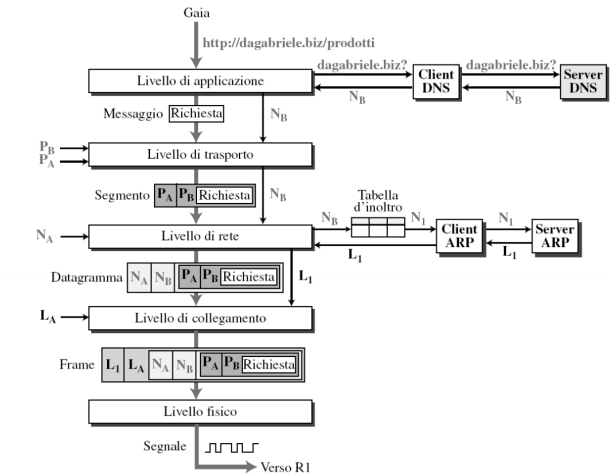
\includegraphics[width=.7\textwidth]{res/flusso-pacchetti-tcpip.png} \hfill
\end{center}